\section{Quantum Spins - 粒子自旋}
We start by motivating \impt{``spin''} as a finite-dimensional degree of freedom in quantum mechanics. \\
We have the following observations:
\begin{quote}
    1. Consider the spectral analysis of quantum systems, with Hamiltonians invariant on rotations (rotationally invariant), and the rotation is $R \in SO(3)$, we see a spectrum of energy levels $\{E_i\}$. As soon as we start working with a Hamiltonian that is \impt{not rotationally invariant}, then each of the previously observed energy levels $E_i$ will be split into $2j+1$ levels (finitely many), where $j \in \{0, \frac{1}{2}, 1, \frac{3}{2}, \dots\}$. This is in the premise of:
    $$SO(3) = \{R \in \R^{3 \times 3} \mid R^{\top}R = RR^{\top} = \id, \det(R) = 1\}$$
    This represents all rotations in 3D space. $S$ means ``special'', $O$ means ``orthogonal''. \\
    2. For Stern-Gerlach, without the magnet, the particle shot out with energy $E$ would only have one energy level, with rotational invariance around the beam axis. However, with a magnet, the Hamiltonian is no longer rotationally invariant around the beam axis, so the energy level splits into $2j+1, j=\frac{1}{2}$ levels.
\end{quote}
The intermediate conclusion from these observations that:
\begin{quote}
    1. Depending on the particle, there exists an additional finite-dimensional degree of freedom that needs to be described. \\
    2. It becomes visible (physically relevant) if the setting is not symmetric under rotations $\iff$ if the setting is rotationally invariant, this degree of freedom is a \impt{conserved quantity}. \\
    3. The conserved quantity associated with rotational invariance (N\"other's theorem) is \impt{angular momentum} ($\hat{\vec{L}} = \hat{\oppos} \times \hat{\opmtm}$). So ``spin'' is ``some sort of'' angular momentum, and its unit is equal to $[\vec{L}] = [\hbar]$. \\
    4. In order to investigate spin, we must investigate how quantum systems and states transform under 3D rotations.
\end{quote}
It is important to distinguish between physical settings and their corresponding mathematical descriptions. In this case, a transformation in the physical space in mathematical representation is unitary representations of groups on $\hilbert$.
\begin{definition}
    Let $G$ be a group and $\hilbert$ be a Hilbert space. \uimpt{A unitary representation} of $G$ on $\hilbert$ is the map
    $$\mathfrak{U}: G \to \text{GeneralLinearOperator}(\hilbert) := \{A:\hilbert \to \hilbert \mid A \text{ is linear and invertible}\}$$
    such that
    \begin{quote}
        1. $\mathfrak{U}(g)$ is a linear operator on $\hilbert$. (Being well-defined) \\
        2. $\mathfrak{U}(g_1g_2) = \mathfrak{U}(g_1)\mathfrak{U}(g_2)$. (Homomorphism) \\
        3. $\conjt{\mathfrak{U}(g)} = \mathfrak{U}(g)^{-1}$. (Unitary)
    \end{quote}
\end{definition}
Take $G = SO(3)$ and $\hilbert = \hilbert_{x_1} \otimes \hilbert_{x_2} \otimes \hilbert_{x_3}$ as an example. Let $\ketpsi \in \hilbert$, with position wavefunction $\psi(\vec{x})$, a trivial representation would be $\forall R \in SO(3), \urep(R) = \id$. Then, in general,
\begin{align*}
    \urep: SO(3) &\to GL(\hilbert) \text{ with } \psi(\vec{x}) \mapsto \psi(R^{-1}\vec{x}) \\
    R &\mapsto \urep(R)
\end{align*}
is a unitary representation of $SO(3)$ on $\hilbert$. \\
We are only interested in the representations that act non-trivially on the full $\hilbert$ space. These representations are considered \impt{irreducible}. Turns out, there is exactly $1$ finite-dimensional irreducible representation for each dimension. These irreducible unitary representations of $SO(3)$ in finite dimensions are the following:
\begin{align*}
    \C^1 \cong \mathcal{D}_0 &: \urep(R) = \id, \text{ scalar, spin-}0 \\
    \C^2 \cong \mathcal{D}_\frac{1}{2} &: \urep(R) = \exp(-\frac{\imag \theta}{2}(e_1X + e_2Y + e_3Z)), \text{ spinor, spin-}\frac{1}{2} \\
    \C^3 \cong \mathcal{D}_1 &: \urep(R) = R, \text{ vector, spin-}1 \\
    \C^4 \cong \mathcal{D}_\frac{3}{2} &: \text{ spin-}\frac{3}{2} \\
    \C^5 \cong \mathcal{D}_2 &: \text{ tensor, spin-}2
\end{align*}
The $\mathcal{D}$ is the representation. \\
It concludes that the Hilbert space of spin-$j$ in 3D space is:
$$\hamiltonian_{\text{tot}} = \hilbert_{x_1} \otimes \hilbert_{x_2} \otimes \hilbert_{x_3} \otimes \mathcal{D}_j$$
and under $R \in SO(3)$ the transformation is:
$$\psi(\vec{x}) \cdot \phi \mapsto \psi(R^{-1}\vec{x}) \cdot \urep(R)\phi$$
Scalars, vectors, and tensors are odd-dimensional representation of $SO(3)$ (classical), while spin-$\frac{1}{2}$ and spin-$\frac{3}{2}$ are representations only of $SU(2)$. $SO(3)$ and $SU(2)$ differ by:
\begin{quote}
    1. Physical quantities related to direction are described by vectors, whose rotations are described by rotation matrices of $SO(3)$. \\
    2. Some quantities like spin are described by spinors, whose rotations are described by rotation matrices of $SU(2)$.
\end{quote}
Here,
$$SU(2) = \{\opuni \in \C^{2 \times 2} \mid \conjt{\opuni}\opuni = \opuni\conjt{\opuni} = \id, \det\opuni = 1\}$$
To explain the transformation further, take $\urep_{\frac{1}{2}}(R)$ specifically, $R$ is a rotation around $\vec{e}$ and $\abs{\vec{e}} = 1$, about some angle $\theta$.
\begin{definition}
    Spin-$j$ is a $2j+1$ degrees of freedom with unit of angular momentum $[\hbar]$ and corresponds to an observable:
    $$\hat{\vec{S}} = \begin{pmatrix}
        \hat{S}_x \\ \hat{S}_y \\ \hat{S}_z
    \end{pmatrix}$$
\end{definition}
For spin-$\frac{1}{2}$, the observable is specifically:
$$\hat{\vec{S}} = \frac{\hbar}{2}\begin{pmatrix}
    X \\ Y \\ Z
\end{pmatrix}$$
Some spin-$j$ particles have an associated magnetic moment. First consider a general angular momentum graph:
\begin{center}
    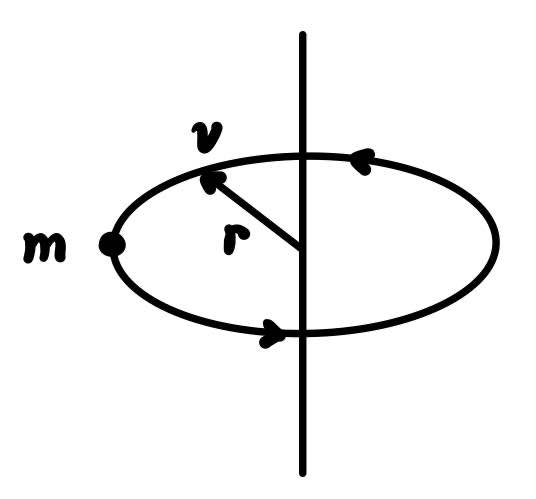
\includegraphics[scale = 0.25]{spin-angular-mtm.jpg}
\end{center}
We have $\abs{\vec{L}} = \abs{\vec{x} \times \vec{p}} = r \cdot m \cdot v$. If charged, it will behave as a magnetic moment $\vec{\mu}$:
$$\vec{\mu} = -\frac{g_s \cdot \mu_B}{\hbar} \cdot \hat{\vec{S}}$$
where $g_s$ is the gyromagnetic factor (different dependent on the particle), and $\mu_B$ is the Bohr magneton $\frac{e \cdot \hbar}{2m_e} \approx 9.3 \text{ J/T}$.

\subsection{Bosons and Fermions - 玻色子和费米子}
\begin{definition}
    Particles with integer spin ($j = 0, 1, 2, \dots$) are \uimpt{bosons}. \\
    Particles with half-integer spin ($j = \frac{1}{2}, \frac{3}{2}, \dots$) are \uimpt{fermions}.
\end{definition}
Some examples of bosons are: photons (spin-$1$), $\Omega$ and $Z$ bosons, Higgs bosons, gluons; some examples of fermions are: photons, neutrons, electrons, quarks, and $\nu$.
\begin{theorem}
    \uimpt{Pauli Exclusion Principle} states that no $2$ fermions in a quantum system can have the same quantum state.
\end{theorem}

\newpage